% Q5V4: Satellite through roof — Signal path diagram
% Satellite → air → roof (concrete) → indoor receiver
\documentclass[border=10pt]{standalone}
\usepackage{tikz}
\usepackage{amsmath}
\usetikzlibrary{arrows.meta, decorations.pathreplacing}
\renewcommand{\familydefault}{\sfdefault}

\begin{document}
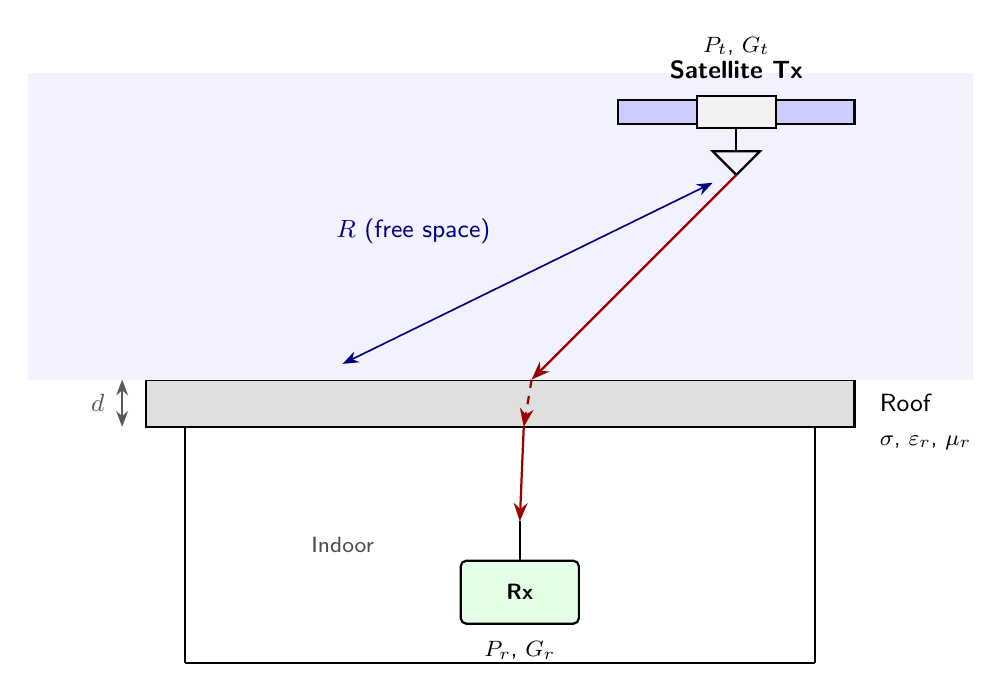
\begin{tikzpicture}[
    every node/.style={font=\sffamily},
    >=Stealth,
]

% === Building structure ===
% Walls
\draw[thick] (2, 0) -- (2, 3);
\draw[thick] (10, 0) -- (10, 3);
% Floor
\draw[thick] (2, 0) -- (10, 0);

% === Roof (concrete slab) ===
\fill[gray!25, draw=black, line width=0.8pt]
    (1.5, 3) rectangle (10.5, 3.6);
\node[right, font=\sffamily\small] at (10.7, 3.3) {Roof};
\node[right, font=\sffamily\footnotesize] at (10.7, 2.8) {$\sigma$, $\varepsilon_r$, $\mu_r$};

% Roof thickness dimension
\draw[<->, line width=0.6pt, gray!70!black] (1.2, 3) -- (1.2, 3.6);
\node[left, font=\sffamily\small, gray!70!black] at (1.1, 3.3) {$d$};

% === Sky region ===
\fill[blue!5] (0, 3.6) rectangle (12, 7.5);

% === Satellite (Tx, upper right) ===
% Satellite body
\draw[thick, fill=gray!10] (8.5, 6.8) rectangle (9.5, 7.2);
% Solar panels
\draw[thick, fill=blue!20] (7.5, 6.85) rectangle (8.5, 7.15);
\draw[thick, fill=blue!20] (9.5, 6.85) rectangle (10.5, 7.15);
% Antenna
\draw[thick] (9.0, 6.8) -- (9.0, 6.5);
\draw[thick] (8.7, 6.5) -- (9.0, 6.2) -- (9.3, 6.5) -- cycle;
\node[above, font=\sffamily\small\bfseries] at (9.0, 7.3) {Satellite Tx};
\node[above, font=\sffamily\footnotesize] at (9.0, 7.6) {$P_t$, $G_t$};

% === Indoor receiver (Rx) ===
\draw[thick, rounded corners=2pt, fill=green!10] (5.5, 0.5) rectangle (7.0, 1.3);
\node[font=\sffamily\footnotesize\bfseries] at (6.25, 0.9) {Rx};
\node[below, font=\sffamily\footnotesize] at (6.25, 0.4) {$P_r$, $G_r$};
% Antenna stub
\draw[thick] (6.25, 1.3) -- (6.25, 1.8);

% === Signal path ===
% Air path (satellite → roof top)
\draw[->, thick, red!60!black] (9.0, 6.2) -- (6.4, 3.6);
% Through roof (dashed)
\draw[->, thick, red!60!black, dashed] (6.4, 3.6) -- (6.3, 3.0);
% Indoor (to receiver)
\draw[->, thick, red!60!black] (6.3, 3.0) -- (6.25, 1.8);

% === Free-space distance ===
\draw[<->, line width=0.6pt, blue!50!black] (4, 3.8) -- (8.7, 6.1);
\node[above left, font=\sffamily\small, blue!50!black] at (6.0, 5.2) {$R$ (free space)};

% === Indoor label ===
\node[font=\sffamily\footnotesize, gray!60!black] at (4, 1.5) {Indoor};

\end{tikzpicture}
\end{document}
